\documentclass[border=2pt]{standalone}
\usepackage{pgfplots}\pgfplotsset{compat=1.17}
\begin{document}
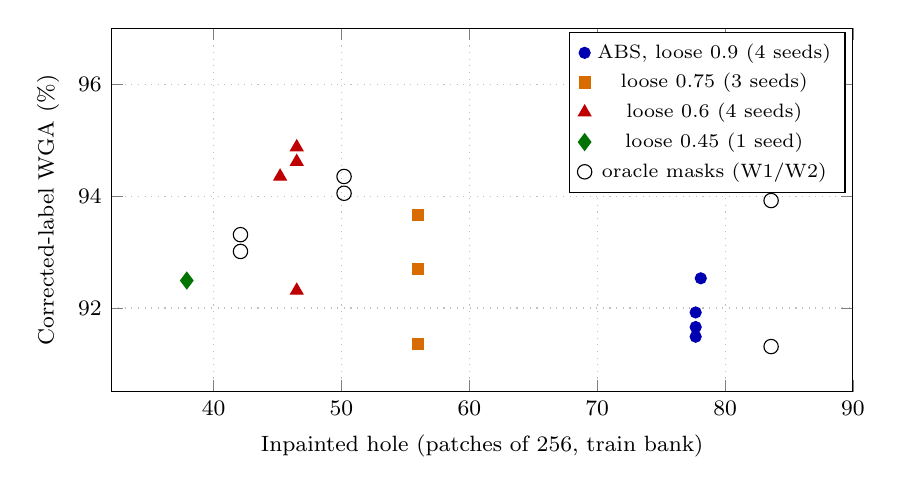
\begin{tikzpicture}
\begin{axis}[width=11cm,height=6.2cm,xlabel={Inpainted hole (patches of 256, train bank)},ylabel={Corrected-label WGA (\%)},
 xmin=32,xmax=90,ymin=90.5,ymax=97,grid=major,grid style={dotted,gray!50},legend style={font=\scriptsize,at={(0.99,0.99)},anchor=north east},
 tick label style={font=\footnotesize},label style={font=\footnotesize}]
\addplot[only marks,mark=*,mark size=2pt,blue!70!black] coordinates {(77.7,91.920)(77.7,91.486)(77.7,91.659)(78.1,92.53)};
\addlegendentry{ABS, loose 0.9 (4 seeds)}
\addplot[only marks,mark=square*,mark size=2pt,orange!85!black] coordinates {(56.0,93.658)(56.0,92.702)(56.0,91.355)};
\addlegendentry{loose 0.75 (3 seeds)}
\addplot[only marks,mark=triangle*,mark size=2.6pt,red!75!black] coordinates {(46.5,94.613)(46.5,92.311)(46.5,94.874)(45.2,94.35)};
\addlegendentry{loose 0.6 (4 seeds)}
\addplot[only marks,mark=diamond*,mark size=3pt,green!45!black] coordinates {(37.9,92.49)};
\addlegendentry{loose 0.45 (1 seed)}
\addplot[only marks,mark=o,mark size=2.6pt,black] coordinates {(50.2,94.05)(50.2,94.35)(42.1,93.31)(42.1,93.01)(83.6,91.31)(83.6,93.92)};
\addlegendentry{oracle masks (W1/W2)}
\end{axis}
\end{tikzpicture}
\end{document}
